\chapter{System Concept}\label{chap:concept}
The following chapter will cover the system concept, the functionality it offers and the general functional system description. Also, the following sections should clarify how the SmartNotes application can be used, illustrate its design using the UML diagrams and prepare the reader for more detailed system description included in the chapter~\ref{chap:sys_description}.

The idea of SmartNotes has been inspired by the Google Notebook application which was being actively developed until January 2009, when Google announced that further development work on this project is stopped. Google Notebook has an interesting interface and features, some of them already motioned in section~\ref{subsec:google_notebook}. what was still missing from the functionality until January 2009 was comfortable notes usage without network connectivity. The aim of the subject of the thesis was to use the idea of making a truly scalable notes taking application that would be even more flexible.

\section{Functionality description}\label{sec:functionality_descr} 
Detailed description of how a system may be used should by of utmost importance both to the developer and to the end user, as it helps gain a general perspective, called 10,000-foot view\cite[page 49]{uml_use_case}, of the system and make useful observations. The implementation as well as the conceptual and system design decisions become a side issue, as the foreground is always occupied by the functionality  the application is to offer. For that reason, the use of case scenarios and flow charts will be very helpful in describing the efficient way of using the SmartNotes application.

Users willing to work on their notes disregarding network connectivity will need to install iSmartNotes, which is a graphical interface of SmartNotes. Specifically, the SmartNotes application is divided into the web-based system and the graphical desktop interface, a separation with which UI experiments can be done without the need of having the web browser open in order to work on the notes. The web based part of SmartNotes makes the synchronization feature possible and allows to monitor the entire system of SmartNotes. However, in order to use the synchronization feature, the iSmartNotes needs to be activated by the user. Additionally, since users of SmartNotes are expected to have a Google account\footnote{Creating a Google account by visiting \url{https://www.google.com/accounts/} gives a access to various services offered by the Google company where Gmail, Google News or Google Finance are one of the most popular tools. These are regarded secure and solid services users can relay on.} the activation code will be available after logging in to the SmartNotes system with that account. This process is illustrated on figure~\ref{fig:ismartnotes_activation}. The idea behind it is to make the use of the popular Google Account and not multiply the accounts to services that the user has to know the login and password. Basing on the activation key, the user is granted access to his personalized SmartNotes account and to the synchronization feature. Without the activation, iSmartNotes can be used as a regular notes editor.  
\begin{figure}[ht]
\begin{center}
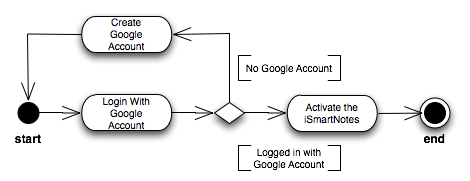
\includegraphics[scale=0.65]{charts/activate_iSmartNotes.png}
\caption{The iSmartNotes application activation with the Google Account.}
\label{fig:ismartnotes_activation}
\end{center}
\end{figure}
The skim of functionality offered by iSmartNotes is demonstrated on figure~\ref{fig:workon_ismartnotes}.
\begin{figure}[ht]
\begin{center}
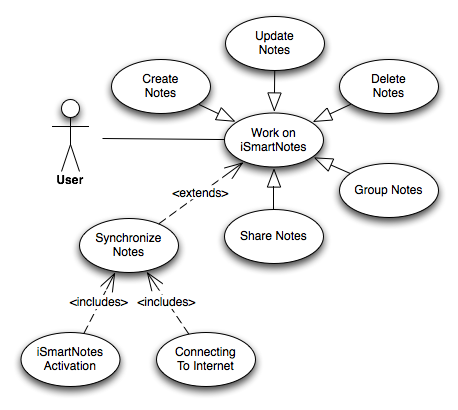
\includegraphics[scale=0.55]{charts/work_on_iSmartNotes.png}
\caption{The iSmartNotes application use cases.}
\label{fig:workon_ismartnotes}
\end{center}
\end{figure}
This includes the CRUD operations and three extra features. Firstly, the notes can be easily grouped together in named tabs, which should make organizing and finding notes much easier. Secondly, it is possible to publish the notes marked as shared. The final feature is the synchronization process that requires iSmartNotes activation and network connection to contact with the web-based part of SmartNotes. What remains to be discussed is the cooperation between iSmartNotes and the web-based part of SmartNotes, therefore, the relation between them and the functionality offered to the user and administrator are shown on figure~\ref{fig:ismartnotes_smartnotes}. 
\begin{figure}[ht]
\begin{center}
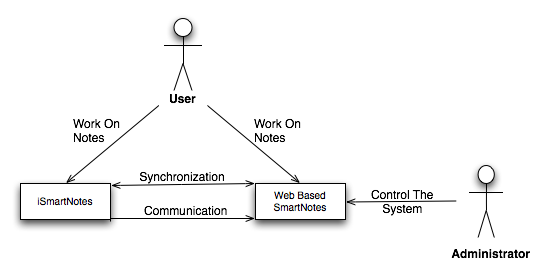
\includegraphics[scale=0.55]{charts/iSmartNotes_SmartNotes.png}
\caption{The cooperation of iSmartNotes and web based SmartNotes.}
\label{fig:ismartnotes_smartnotes}
\end{center}
\end{figure}

This interesting concept allows the user to work on iSmartNotes as well as the Web-based part of SmartNotes exchangeably, at the same time letting the SmartNotes application care for work synchronization, which has been also highlighted in the above discussed picture. Yet, however functional and elastic the application may seem, the same functionality is not feasible in the web interface of the present project, even if the administrator is granted access to tools like datastore data browser, system status or application dashboard described in section~\ref{sec:gae_general}. This can help to quickly diagnose faults within the application and rollback it to the latest stable version. Moreover,  it can indicate that the rescuers are not sufficient to serve the traffic and eventually extend them. The tools work effectively in cooperation with Google Webmaster Tools and the Google Analytics as they can provide more information concerning the web page and its visitors.

It appears to be worth describing the synchronization feature in more detail. The feature is realized by the VCS which was introduced in section~\ref{sec:popular_vcs}. No matter if the user works online or not, they have full access to notes and synchronize them online. As it has been marked on the graph from figure~\ref{fig:ismartnotes_smartnotes}, the synchronization process is bidirectional: it is triggered from the web-based part of SmartNotes, which plays a role of the main server, and the iSmartNotes, playnig the role of clients and reverse. This type of set-up should allow to update the notes whenever necessary. Another point presented in figure~\ref{fig:ismartnotes_smartnotes} is the directional communication between iSmartNotes and SmartNotes, which should be understand as an additional logic allowing to perform operations on the user side by the help of iSmartNotes, including the display of user information on significant events like availability of new features or versions.  As a matter of fact, the process is directional in one way as it is the iSmartNotes application which receives the information from the SmartNotes server and displays it to the user. Whereas the presented functionality does not fully exploit the possible feature list, as mentioned in section~\ref{subsec:vcs_comparison}, it is a good practice to keep the application as simple as possible and focus on a set of clearly defined key features.

\section{Functional description}\label{sec:functional_descr}
The SmartNotes application should run on a infrastructure that can ensure complete availability and high load. Easy system maintenance and openness to future expansion in functionality are also strongly desirable features. It is not pointless to mention that the above requires resource usage, which makes the financial model of utmost importance and is the already introduced 10,000-foot view of system requirements. Adding a friendly deployment methodology and good documentation is what would satisfy the most demanding developer.

Admittedly, in order for the application to gain popularity, users should be well informed about the application and its functionality; also, it is vital to provide availability of instructions on how to get started. For these reasons, the landing page should be not only informal and practical, but also international to reach greater group of users.

From the architectural point of view, SmartNotes is a simple client-server application, the only difference being the usage of DVCS, which allows the machines to access thesame set of commands and make their hard disks hold the entire repository with its history. Yet, it may be confusing that it still remains a client-server architecture, but just as the centralized VCS do not recognize any other architecture than the client server, the distributed VCS uses it as one of possible use cases. In the following scenario one of the machines fulfills a role of the reverential server to which all remaining machines direct their requests, at the same time being a for of public repository with the most recent version that should be always available to users. In consequence, each client requires the installation of DVCS as one of the main components, while the size of the chosen VCS matters as much as its performance, which all in all has significant impact on the final performance of iSmartNotes. For optimum user experience, the iSmartNotes application provides an easy-to-install package that could be downloaded from the server serving static content, which is not only a faster solution from dynamically served content, but also allows to save system resources, costing a minimum of CPU time.

The next two sections state certain problems related to synchronization scenarios using VCS and the application activation. They will be analyzed focusing on the evaluating of a number of possible solutions and the argumentation will lead to the choice of the most optimal solution.  
 
\subsection{Synchronization scenarios using version control systems}\label{subsec:sync_scenarios}
It is one of the main responsibilities of Version Control Systems to keep the repositories updated. Nevertheless, they never perform an update without a user request\footnote{This means that the user has to run an appropriate command or click on the right button when using a graphical interface. It could be naturally automated by writing a script that would perform that task for the user or by setting a cron job with a desired time interval, but the tool still requires the user to trigger the update process.}, the reasons for which are various, but dealing with conflict situations like the one shown on figure~\ref{fig:google_notebook} seams to be the most important. To put it in simple words conflict situation it is a situation when the VCS needs the user decision to resolve the conflict situation as it cant decide which from the concurring versions should be chosen. The way the merging is done differs with different Version Control Systems, but from the user perspective, operations such as update and merge are relatively easy to imagine. 

Due to the lack of clarity in terminology regarding basic operations of Version Control, additional explanations seem to be required. Mercurial implements the \texttt{fetch} command  which includes three steps listed in the order of execution:
\begin{enumerate}
\item{Lookup.}
\item{Getting changesets\footnote{The term used mainly in Mercurial-related documentation to refer to data structures used for storing the differences between revisions. These seem to be more accurate then the basic notions of 'changes' or 'differences' and will be used in this document when concerning data structures.}.}
\item{Updating or merging.}
\end{enumerate}
The first two steps are implemented by Mercurial as \texttt{pull} command,whereas the third one has two commands called \texttt{update} and \texttt{merge} respectively. On the other side in the git system, \texttt{fetch} does the same as Mercurial \texttt{pull} command and the git \texttt{pull} is a substitute for the \texttt{fetch} from Mercurial. To avoid confusion, terminology used in the git system only will be used in the present thesis.

iSmartNotes needs to enable three functional operations: 
\begin{itemize}
\item{Update -- retrieving newer versions from the main server, or down-side synchronization.}
\item{Apply changes -- operations of creating, updating and removing content.}
\item{Synchronize -- up-side synchronization to the main server.}
\end{itemize}
All of the above are essential to realize the full set of iSmartNotes use cases, which were generalized under the term \textit{Work on iSmartNotes} on figure~\ref{fig:workon_ismartnotes}. The sequence diagrams~\ref{fig:seq_update},~\ref{fig:seq_commit} and~\ref{fig:seq_commit2}  demonstrate how these operations could be decomposed into lower level calls. The operation of applying changes and synchronizing has been presented in one sequence as all of the sequences make an assumption of network connectivity, which allows to join them easily. It must be noted that without such a system, the operations are much more simple as they become limited to the interaction between client repository the application (the terms 'client' and 'server' being used intentionally instead of the application-specific names in order to stress the client-server architecture and make the examples more general).

The first of the diagrams illustrates internal relation of operations needed to perform the pull operation. Additionally, the order in which these operations are being executed can be observed by reading the sequence diagrams from top to bottom.
\begin{figure}[ht]
\begin{center}
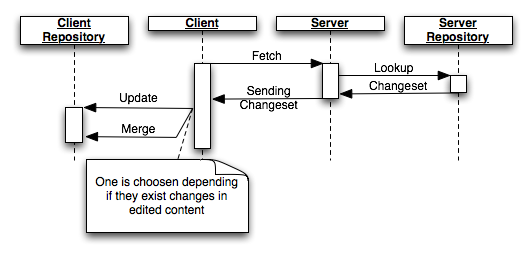
\includegraphics[scale=0.6]{charts/seq_update.png}
\caption{The pull operation sequence diagram.}
\label{fig:seq_update}
\end{center}
\end{figure}
The operation is started by the client by requesting changesets from the server and finishes after update or merge operation is performed on the client repository. As noted on figure~\ref{fig:seq_update}, the condition deciding which of them should be chosen depends on the existence of changes in the edited content. If merging is not required, then the update operation is performed, whereas when no chengsets are found, then none of the above is needed. That is a general rule when choosing between merge and update and for this reason, the fact will not be repeated on the following figures. It is also common that on the sequence diagrams, client and server repository are separated from their Version Control repositories and it is thanks to this concept that the front-end and back-end functions may be presented simultaneously. 

Figures~\ref{fig:seq_commit} and~\ref{fig:seq_commit2} are the product of dissertation on what sequence the operations should be called to receive a updated version after applying changes. The first one illustrates the idea of performing a \texttt{pull} first after the changes are saved in the clients repository and the \texttt{push} at the end of the sequence. The opposite order is presented on figure~\ref{fig:seq_commit2} where \texttt{pull} is followed by \texttt{push}. 
\begin{figure}[ht]
\begin{center}
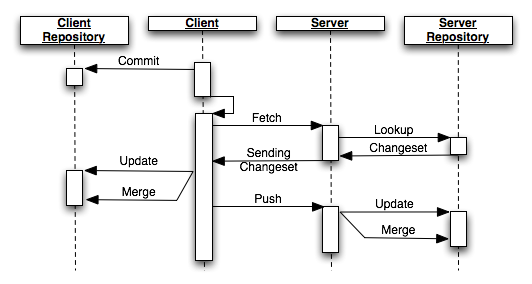
\includegraphics[scale=0.6]{charts/seq_commit.png}
\caption{The commit operation together with pull preceding the push operation.}
\label{fig:seq_commit}
\end{center}
\end{figure}
\begin{figure}[ht]
\begin{center}
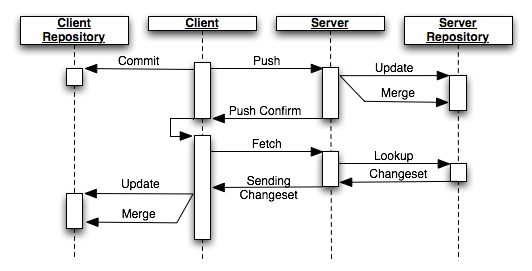
\includegraphics[scale=0.6]{charts/seq_commit2.png}
\caption{The commit operation that makes push follow the pull operation.}
\label{fig:seq_commit2}
\end{center}
\end{figure}
\newline Both of those attempts have its advantages and disadvantages. On balance, the first concept appears to outperform the second one by the following characteristics:
\begin{itemize}
\item{The basic client action is finished faster as it only saves the changes in the client repository.}
\item{Lower probability that the server will need to perform the merge operation, which allows to save CPU resources and makes the application more scalable as the merges are completed on the client application side. The latter also solves potential conflicts before the changesets reach the server.}
\item{Better user experience; effectively, changes are available in the interface offered by the client application sooner.}
\end{itemize}
On the other hand, the second concept may seem more reliable as it gives greater priority to saving changesets both in the client and the server repositories and preforms commit and \texttt{push} as the first action. Yet, the latter fails to make significant difference in practice and is easily outweighed by the arguments mentioned above. One additional motion that can be taken is that the processes used by VCS are more complicated that they may look from the user perspective. More the the processes that were presented on figures~\ref{fig:seq_update},~\ref{fig:seq_commit} and~\ref{fig:seq_commit2} are only the top level operations which have their own logic and set of communicates that are build of.

\subsection{iSmartNotes activation process}\label{subsec:ismartnotes_activation}
Most of network applications that require account credentials for each of their users actually create the new account, which causes uncomfortable situation to users willing to use the application with numerous logins and passwords that require security. The latter is frequently provided by various password managers storing thie data on the local machine and preventing the user from remembering all of them. That mechanisms are definitely helpful, however, in case the user changes the machine, they will be prompted for the login and password again. Then, is there any solution? Recently, interesting work has been done with OAuth, yet its plain format is limited to web-based applications and cannot be used for authenticating non-web-based applications. Because one of the aims of SmartNotes was to simplify the usage of the application to the maximum, solving this particular problem was significant. Obviously, creating a classical user account was not a perfect solution as by adding that, the iSmartNotes interface, in the future an internationalized one, might require other options that in the classical case would require the user to set them in the preferences. When it does not remain a problem to one group of users, others might find that functionality highly dissatisfying, therefore, bearing that in mind, the perfect solution would be allow the user to download a perfectly personalized application with all of the above functionality already configured. That would mean the user could start to use the application just after it has been downloaded, which eventually is an ideal situation. Moreover, it is not trivial to realize the same when taking into account that the application should stay scalable and be seamlessly downloaded as a static file. Building the application per user would cost CPU time and require to have certain software installed on the server where the application is hosted. Then, what could be considered as conceptual compromise is creating one account and using its setting with for all other services that require authentication. This application could provide basic personal information that could be used by the applications, e.g. the language setting, which could be easily changed once and used for all tools available in the application. This is not yet implemented by the Google Account, which currently provides a secure mechanism for user authentication with the login and password they use to log to any of the Google services. The developer has access to the user ID, mail address and nickname of the authenticated user. However, this mechanism is limited only to web applications and requiring the Google Account credentials directly from the application remains out of question. All in all, one of the possible solutions is to use a serialized data in the activation code and the construction of such an activation code is presented on figure~\ref{}. It has three main parts:
\begin{itemize}
\item{Password. Randomly generated string.}
\item{Userid. The userid from the Google Account, which stays the same even if a change of email address is performed.}
\item{Account data. This should be a data structure allowing to store some simple informations like when the user started to use the application or internationalization settings.}
\end{itemize}
All these elements should be serialized into a single string which could be used as the activation key by iSmartNotes. Therefore, no matter if the user decides to use iSmartNotes for the first time or has just changed the machine, they will only be required to login to SmartNotes using their Google Account, download the application and pass the activation code. To make an even more conspicuous comparison between this idea and its performance based on a classical account system, figure~\ref{} demonstrates the actions that the user has to follow to use the systems. Yet, the fact that it becomes a standard for network applications and more and more users know this procedure does not make it a perfect solution. In this case, just like for choosing the best synchronization scenario, there will be chosen the optimal concept in terms of its implementation; specifically, the activation code seems to be the best compromise between low user complication level and system complexity and cost.
